% This is samplepaper.tex, a sample chapter demonstrating the
% LLNCS macro package for Springer Computer Science proceedings;
% Version 2.20 of 2017/10/04
%
\documentclass[runningheads]{llncs}
%
\usepackage{graphicx}
% Used for displaying a sample figure. If possible, figure files should
% be included in EPS format.
%
% If you use the Hyperref package, please uncomment the following line
% to display URLs in blue roman font according to Springer's eBook style:
% \renewcommand\UrlFont{\color{blue}\rmfamily}

\usepackage{orcidlink} % Orcid links
% Fix underscore in dois
\usepackage[strings]{underscore}

% Listing settings
\usepackage{listings}
\usepackage{xcolor}

\lstdefinelanguage{Interaction}[]{Java}{
    comment=[l]{---},
}

\lstset{emph={
    synchronize
    },emphstyle={\color{blue}\bfseries}
}

\begin{document}
% https://www.discotec.org/2024/coordination
% Regular papers 7-15 pages + references
% Artifacts using Zenodo together with this repo. Maybe a big CSV file with our classification results is input for some plots (clustering). Then, the source code for that should also be added.
\title{Classifying coordination approaches}
%
%\titlerunning{Abbreviated paper title}
% If the paper title is too long for the running head, you can set
% an abbreviated paper title here
%
\author{Tim Kr\"{a}uter\inst{1}\orcidlink{0000-0003-1795-0611} \and
Julien Deantoni\inst{2}\orcidlink{0000-0001-6962-7846}
Adrian Rutle\inst{1}\orcidlink{0000-0002-4158-1644} \and
Harald K\"{o}nig\inst{3,1}\orcidlink{0000-0001-6304-6311} \and
Yngve Lamo\inst{1}\orcidlink{0000-0001-9196-1779}}
%
\authorrunning{T. Kräuter et al.}
% First names are abbreviated in the running head.
% If there are more than two authors, 'et al.' is used.
\institute{Western Norway University of Applied Sciences, Bergen, Norway  \\
\email{tkra@hvl.no, aru@hvl.no, yla@hvl.no} \and
University Cote d’Azur, Sophia Antipolis, France \\
\email{julien.deantoni@univ-cotedazur.fr} \and
University of Applied Sciences, FHDW, Hanover, Germany\\
\email{harald.koenig@fhdw.de}}
%
\maketitle              % typeset the header of the contribution
%
\begin{abstract}
TODO
\keywords{
ADL \and
Coordination language \and
Coordination framework \and
Co-Simulation \and
Feature model
}
\end{abstract}

\section{Introduction} \label{sec:introduction}

% Categorizing ADLs, Coordination languages, Co-simulation, and Coordination frameworks (BCOOL and me).

% Paper outline

% What was our search methodology? Google Scholar? Other databases? Which search terms/queries?

\section{Categories of Coordination Approaches} \label{sec:approaches}

\autoref{fig:overview} gives an overview of the different categories of coordination approaches.
% TODO: Describe the overview layer/level by level.

\begin{figure}[ht]
	\centering
	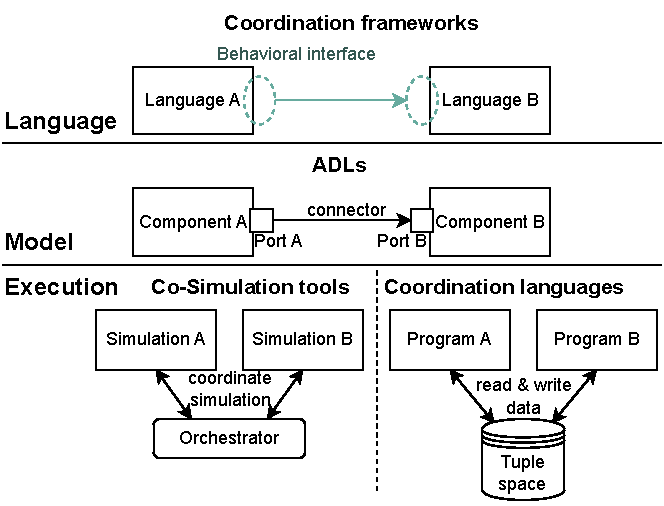
\includegraphics[width=0.7\textwidth]{images/overview}
	\caption{Overview of coordination approaches}
	\label{fig:overview}
\end{figure}

In the following sections, we will describe each of the categories: ADLs, coordination languages, Co-Simulation tools, and coordination frameworks in detail.

\subsection{Architecture Description Languages}
% Define ADL and give examples.
% Which ADLs are we interested in?
% Not all of them since some such as ArchiMate are just for diagramming? --> Our definition should exclude archimate.
% Cite ADLs and a survey about them.

% Nice for definitions: components, connectors and configurations
\cite{medvidovicFrameworkClassifyingComparing1997}


% Nice for definitions (Bold terms in the categorization): components, connectors and configurations
% "No ADL provides explicit support for multiple formal specification languages."
\cite{medvidovicClassificationComparisonFramework2000}

% Nicely outlines the overlap between requirements languages, programming languages, modeling languages and ADLs. --> Good sentence for adls are not clearly defined and overlap with other languages
% "There is no clear line between ADLs and non-ADLs"
% Commonaltities listed are nice: formally-defined semantics, lack of real-world applications <.<
\cite{clementsSurveyArchitectureDescription1996}

% "ADLs are still not mainstream, i.e., used by practioners."
% Good description of ADLs such as Darwin, Wright with citations and examples.
% "ADLs usually use process algebras which practionoers do not like"
\cite{ozkayaAreWeThere2013}


% ADLs vanished but UML didnt which people did not accept as an ADL!
% In academia ADL have to allow for some formal analysis or something, which UML doesnt. We stick to the academic definition and do not consider UML or Archimate as ADLs in this paper. But yeah both languages are used heavily to describe software architectures.
\cite{pandeyArchitecturalDescriptionLanguages2010}

\subsection{Coordination Languages}
% Define Coordination language and give examples
% Cite and survey

\subsection{Co-Simulation Tools}
% Define Co-Simulation and give examples
\cite{gomesCoSimulationSurvey2019}

\subsection{Coordination Frameworks}
% Define Coordination-framework and give examples
% Cite and survey?
\cite{varalarsenBCOolBehavioralCoordination2016,varalarsenBehavioralCoordinationOperator2015}~\cite{krauterBehavioralConsistencyMultimodeling2023}

% Maybe add the overview from Julien and me here to help with the definition

\section{Feature model} \label{sec:features}
% Cut up the feature model and describe it in dedicated subsections (maybe the first layer of nodes after the root)
% Maybe add a full feature model as an artifact (use GitHub repo with Zenodo)

\begin{figure}[ht]
	\centering
	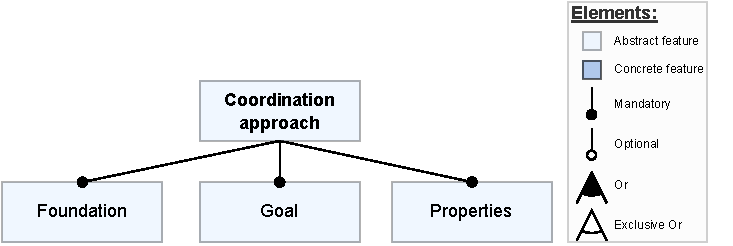
\includegraphics[width=1\textwidth]{images/root}
	\caption{Feature Model Overview}
	\label{fig:feature_model_root}
\end{figure}

\subsection{Coordination}
\subsection{Goal}
\subsection{Properties}

\section{Classification examples} \label{sec:classifications}

% Classify some representatives, sticking to the same order as in the preliminaries.
\subsection{MontiArc} % ADL representative
\subsection{Lingua Franca} % Coordination language representative
\subsection{Co-Simulation example} % Co-Simulation representative
\subsection{BCOOL} % Coordination framework representative
\subsection{BCorrLang} % Coordination framework representative --> Need to classify my approach for the thesis

\section{Classification results}
% Clusters of features for ADL, Coordination language, Co-Simulation, and coordination frameworks?
% Maybe they can somehow be visualized nicely using some clusters with overlaps (vann diagram or something)

% Commonalities between clusters

% Differences between clusters

% What are the unique features of each approach? Does this match their intended usage scenarios?

\section{Running example}
% I'm not sure about this section yet, but a running example would be nice to show in different approaches.

\lstinputlisting[
label=lst:interactions,
language=Interaction,
caption=Interactions for the running example]{listings/interactions.txt}

\section{Conclusion} \label{sec:conclusion}

\bibliographystyle{splncs04}
\bibliography{bib}

\end{document}
